\documentclass[12pt, oneside]{book}
\usepackage[spanish]{babel}
\usepackage{csquotes}
\usepackage{geometry}
\geometry{
  a4paper,
  left=25.4mm,
  right=25.4mm,
  top=25.4mm,
  bottom=25.4mm,
  }
\usepackage{graphicx}
\usepackage{algorithm}
\usepackage{setspace}

\usepackage{UnsaacTitle}
\author{ALEX HARVEY PFOCCORI QUISPE}
\title{GENERACIÓN DE UN DATASET PERSONALIZADO PARA LA DETECCIÓN AUTOMÁTICA DE CASCOS DE SEGURIDAD EN TRABAJADORES DE CONSTRUCCIÓN UTILIZANDO EL MODELO YOLOv8}
\usepackage{graphicx}


\usepackage[
backend=biber,
style=ieee,
]{biblatex}
\addbibresource{bibliography.bib}
% \usepackage{titlesec}
% \titleformat{\chapter}
%   [hang] % Estilo del formato (hace que el título quede alineado)
%   {\normalfont\LARGE\bfseries} % Estilo del texto
%   {CAPÍTULO \thechapter.} % Texto que aparece antes del título (número de capítulo seguido de un punto)
%   {1em} % Espacio entre "CAPÍTULO 1." y el título
%   {\MakeUppercase} % Hace que el título del capítulo esté en mayúsculas


\usepackage[hidelinks]{hyperref}
\linespread{1.25}

\begin{document}
\maketitle

\doublespacing

% Include initial sections
\thispagestyle{plain}
\newpage

\begin{center}
  \textbf{DEDICATORIA}
\end{center}

\vspace{1cm}

A Dios, por darme salud y fortaleza para culminar el presente trabajo de investigación.

A mis padres Gabina y Mauro, quienes me brindaron su apoyo incondicional y estuvieron a mi lado en todo momento, recordándome la importancia de la perseverancia y el esfuerzo. Su amor y fortaleza fueron esenciales para culminar esta etapa de mi vida.

A mi tía Roxana, a quien considero como mi segunda madre. Su motivación constante y sus palabras de aliento me impulsaron a seguir adelante y a no rendirme hasta alcanzar mi meta. Gracias por creer en mí siempre.

A mi hermano Arnold, quien en todo momento me alentó a continuar con esta investigación, dándome la confianza necesaria para superar cada obstáculo.

A mis hermanas Anai y Adel, cuyas ocurrencias y risas me mantuvieron despierto hasta altas horas de la noche, impulsándome a avanzar en cada capítulo. Gracias por alegrar mis días y por su compañía.

Y a Zaru y Dara, mis queridas mascotas, que con su ternura y dulzura iluminan mis días. Su compañía fue mi refugio en los momentos de agotamiento y estrés.

\vspace{2cm}

\begin{flushright}
  \textbf{\textit{Alex Harvey Pfoccori Quispe}}

  \textbf{\textit{26 de septiembre del 2024}}
\end{flushright}

\newpage
\thispagestyle{plain}

\begin{center}
  \textbf{AGRADECIMIENTOS}
\end{center}

\vspace{1cm}

\noindent

Quiero expresar mi más profundo agradecimiento a todas las personas que han contribuido, de una u otra forma, a la culminación de este trabajo de investigacion.

En primer lugar, agradezco a mis padres, quienes con su amor, apoyo incondicional y sacrificios, han sido mi fuente de motivación y fortaleza a lo largo de este proceso académico. Sin ustedes, este logro no habría sido posible.

A mi tutor Phd. Hans Harley Ccacyahuillca Bejaar, por su dedicación y guía constante. Su conocimiento, orientación y valiosos comentarios han sido fundamentales para la realización de este trabajo. Gracias por compartir su experiencia y por motivarme a ir siempre más allá.

A mis compañeros y amigos, quienes con su apoyo y ánimo me han acompañado en este camino. Sus palabras de aliento y su compañía en los momentos difíciles han sido de gran importancia para mí.

A los trabajadores y responsables de la obra ``Comercio'', por permitirme acceder a las instalaciones y contribuir con las imágenes necesarias para la creación del dataset. Este trabajo es una muestra del compromiso que todos compartimos por mejorar la seguridad en las obras de construcción.

Finalmente, agradezco a Dios por darme la fortaleza y la oportunidad de seguir adelante en este reto.

\vfill

\pagebreak
\thispagestyle{plain}

\newpage

\begin{center}
  \textbf{RESUMEN}
\end{center}

\vspace{1cm}

Esta investigación se centra en la generación de un dataset personalizado para el entrenamiento del modelo de detección de objetos YOLOv8, específicamente para la detección de equipos de protección personal (EPP) en trabajadores de la industria de la construcción. La falta de datasets públicos disponibles con imágenes del mundo real de trabajadores usando EPP motivó la creación de este dataset, el cual fue recolectado en la obra ``Comercio''. Utilizando un celular  de la marca Honor, se capturaron imágenes de 5792x4344 píxeles, que fueron preprocesadas para estandarizar sus dimensiones a 640x640 píxeles para el entrenamiento del YOLOv8.

Se implementaron tres algoritmos de recorte: recorte desde la izquierda, recorte centrado y recorte con superposición. Además, se utilizó el modelo preentrenado de YOLOv8 para detectar personas en las imágenes y se recortaron las áreas de interés en consecuencia. Las imágenes sin personas fueron filtradas usando otras versiones del modelo YOLOv8, obteniendo un dataset final de 642 imágenes recortadas. Se aplicó aumentación de datos para duplicar el tamaño del dataset y las imágenes fueron etiquetadas con la clase \textit{``helmet''}  para la detección de cascos utilizando Roboflow. El dataset final, con 1284 imágenes, se encuentra disponible en la plataforma Roboflow.

\textit{\textbf{Palabras clave:}} Procesamiento de imágenes, detección de objetos, visión por computadora, YOLOv8, seguridad en la construcción.

\vfill

\pagebreak
\thispagestyle{plain}

\newpage

\begin{center}
  \textbf{ABSTRACT}
\end{center}

\vspace{1cm}

This research focuses on the generation of a custom dataset for training the YOLOv8 object detection model, specifically for detecting personal protective equipment (PPE) in construction workers. The lack of publicly available datasets with real-world images of workers using PPE motivated the creation of this dataset, which was collected at the ``Comercio'' construction site. Using an Android smartphone, images of 5792x4344 pixels were captured and preprocessed to standardize their dimensions to 640x640 pixels for YOLOv8 training.

Three image cropping algorithms were implemented: left-side cropping, centered cropping, and overlapping cropping. Additionally, the YOLOv8 pre-trained model was used to detect individuals in the images, and regions of interest were cropped accordingly, the algorithms are in the \href{https://github.com/Aleticod/yolo_image_preprocessing}{GitHub Repository}. Images without people were filtered out using other YOLOv8 model versions, yielding a final dataset of 642 cropped images. Data augmentation was applied to double the dataset size, and the images were labeled for helmet detection using Roboflow. The final dataset, with 1284 images, they are available in Roboflow platform.

\textit{\textbf{Keywords:}} Image processing, object detection, computer vision, YOLOv8, construction safety.

\vfill

\pagebreak
\thispagestyle{plain}

\begin{center}
  \textbf{INTRODUCCION}
\end{center}

\vspace{1cm}

\noindent
En el ámbito de la construcción, la seguridad de los trabajadores es una prioridad fundamental, y el uso adecuado de equipos de protección personal (EPP) es crucial para prevenir accidentes y lesiones. Los cascos de seguridad, juegan un rol vital en la mitigación de riesgos. Sin embargo, a pesar de las regulaciones y normativas que promueven su uso, la supervisión del cumplimiento en tiempo real puede resultar difícil debido a las limitaciones humanas y tecnológicas. Es en este contexto donde las soluciones basadas en visión por computadora y modelos de inteligencia artificial, como YOLOv8, ofrecen un enfoque innovador para mejorar la seguridad en las obras.

YOLOv8 (\textit{You Only Look Once}) es uno de los modelos de detección de objetos más avanzados y precisos, capaz de identificar y localizar objetos en imágenes en tiempo real con alta eficiencia. Sin embargo, el rendimiento de estos modelos depende en gran medida de la calidad y cantidad de los datasets utilizados durante su entrenamiento. Si bien existen diversos datasets públicos, la mayoría están diseñados para entornos controlados y no reflejan adecuadamente las condiciones reales de una obra de construcción. Esto plantea la necesidad de crear un dataset específico que capture a los trabajadores en un entorno real.

Este trabajo de investigación tiene como objetivo principal la generación de un dataset personalizado con imágenes reales tomadas en una obra de construcción, el cual servirá como base para el entrenamiento del modelo YOLOv8. Las imágenes fueron obtenidas en el proyecto "Comercio" utilizando un dispositivo móvil, y posteriormente preprocesadas para cumplir con los estándares requeridos para el entrenamiento del modelo. Además, se desarrollaron distintos algoritmos de recorte y técnicas de filtrado, apoyados por el uso de modelos preentrenados.

La investigación también incluye la aplicación de técnicas de aumentación de datos para expandir el conjunto de imágenes y el etiquetado manual de cascos de seguridad, empleando herramientas como la plataforma Roboflow. El resultado final es un datasetp para el entrenamiento de modelos de detección de EPPs en contextos reales.

\vfill

\pagebreak

% Main content
% \renewcommand{\contentsname}{INDICE}
\tableofcontents

\listoffigures
\newpage

\listoftables
\newpage

% Includes chapters
\chapter{INTRODUCCIÓN}
En el ámbito de la industria de la construcción, garantizar la seguridad de los trabajadores es una tarea de suma importancia, donde el uso correcto de los equipos de protección personal (EPP) es esencial para minimizar accidentes y lesiones. Los cascos de seguridad, entre otros elementos de protección, juegan un papel indispensable en la reducción de riesgos. No obstante, aunque existen normativas que exigen su uso, la supervisión en tiempo real de su cumplimiento es un desafío debido a las limitaciones de los métodos tradicionales de monitoreo. Ante esta problemática, las tecnologías basadas en visión por computadora y modelos de inteligencia artificial, como YOLOv8, ofrecen una alternativa prometedora para optimizar la seguridad en las obras.

YOLOv8, cuyo nombre es un acrónimo de \textit{``You Only Look Once''}, es uno de los modelos más avanzados para la detección de objetos, capaz de identificar y localizar elementos en imágenes en tiempo real con gran precisión y eficiencia. A pesar de sus capacidades, el desempeño de estos modelos está directamente relacionado con la calidad y cantidad de los conjuntos de datos que se utilizan en su entrenamiento. Aunque existen datasets de acceso público, la mayoría están diseñados para entornos controlados y no reflejan con precisión las condiciones reales de una obra. Esto destaca la necesidad de crear un conjunto de datos específico que represente a los trabajadores en condiciones reales usando EPP, particularmente cascos de seguridad.

El presente trabajo tiene como objetivo principal la creación de un dataset personalizado con imágenes capturadas en una obra de construcción real, que será utilizado para entrenar el modelo YOLOv8. Las fotografías fueron tomadas en el proyecto ``Comercio'' con un dispositivo móvil y luego preprocesadas para cumplir con los estándares necesarios para el entrenamiento del modelo. Además, se implementaron diferentes algoritmos de recorte y técnicas de filtrado, utilizando modelos preentrenados para garantizar que las imágenes seleccionadas sean de alta calidad y pertinentes para el objetivo del estudio.

Para complementar el conjunto de datos, se aplicaron técnicas de aumentación de datos con el fin de expandir el número de imágenes disponibles. También se llevó a cabo el etiquetado manual de los cascos de seguridad presentes en las imágenes utilizando herramientas especializadas, como la plataforma Roboflow. El resultado final es un dataset optimizado que permitirá el entrenamiento eficiente de modelos de detección de EPP en escenarios reales.

\section{Generalidades}

El presente trabajo de investigación tiene como objetivo principal la creación de un dataset personalizado para la detección automática de cascos de seguridad en trabajadores de construcción utilizando el modelo de inteligencia artificial YOLOv8. La importancia de este proyecto radica en la necesidad de mejorar la supervisión del uso de equipos de protección personal (EPP) en tiempo real, ya que la seguridad en obras de construcción es un aspecto crítico para la prevención de accidentes.

La base de este trabajo es el desarrollo de un conjunto de imágenes reales capturadas en una obra de construcción, las cuales se han preprocesado y filtrado para cumplir con los requerimientos del modelo YOLOv8. Este modelo es ampliamente reconocido por su capacidad de detectar objetos en tiempo real con alta precisión, lo que lo convierte en una herramienta eficaz para la vigilancia y monitoreo de condiciones laborales seguras.

El proyecto incluye tanto la recolección y preprocesamiento de datos, como la implementación de técnicas de recorte de imágenes, detección de objetos (personas), aumentación de datos y etiquetado de imágenes. Además, se aplican modelos preentrenados de YOLOv8 para el filtrado de las imágenes y garantizar la detección precisa de los cascos de seguridad en las fotografías tomadas en un entorno de obra real.

Este trabajo no solo busca contribuir a la mejora de los sistemas de monitoreo en obras de construcción, sino también ofrecer una referencia útil para futuros estudios y desarrollos relacionados con la seguridad en el ámbito laboral a través de la inteligencia artificial y la visión por computadora.

\section{Planteamiento y Formulacion del Problema}

\subsection{Planteamiento del problema}

En la industria de la construcción, los accidentes laborales continúan siendo una de las principales causas de lesiones graves y fallecimientos. A pesar de la implementación de normativas y la obligatoriedad del uso de equipos de protección personal (EPP), como los cascos de seguridad, el monitoreo efectivo de su uso en tiempo real es limitado. La supervisión manual no es eficiente ni escalable en entornos de trabajo grandes o complejos, lo que conlleva a la necesidad de aplicar nuevas tecnologías para abordar este desafío.

La inteligencia artificial, en particular los modelos de detección de objetos basados en visión por computadora, ha demostrado ser una solución prometedora para la automatización de procesos de seguridad en entornos industriales. Sin embargo, el rendimiento de estos modelos depende en gran medida de la calidad y la relevancia de los datasets utilizados para su entrenamiento. Actualmente, los datasets públicos que contienen imágenes de personas usando EPPs en contextos reales son escasos, y muchos de los disponibles están limitados a entornos controlados, con variaciones limitadas de las condiciones de iluminación, ángulos de visión y contextos laborales.

Este vacío de datasets reales con imágenes de trabajadores usando EPPs en obras de construcción dificulta el desarrollo de soluciones automatizadas eficaces para la detección de equipos de seguridad. Como resultado, es esencial la creación de un dataset personalizado que refleje las condiciones reales de una obra de construcción, permitiendo así entrenar modelos de detección de objetos más precisos y efectivos.

\subsection{Formulación del Problema}

El problema central que aborda este trabajo de investigación es el siguiente:

\textbf{¿Cómo generar un dataset personalizado que permita entrenar de manera eficaz un modelo de detección de objetos (YOLOv8) para identificar el uso de cascos de seguridad en trabajadores de construcción en un entorno real?}

\section{Alcances y Limitaciones}

\subsection{Alcances}

El presente trabajo de tesis se enfoca en la creación de un dataset personalizado para el entrenamiento del modelo YOLOv8, destinado a la detección de cascos de seguridad en trabajadores de una obra de construcción. El alcance de este proyecto comprende lo siguientes:

\begin{itemize}
  \item \textbf{Recolección de imágenes en obra:} Se capturarán imágenes reales de trabajadores utilizando equipos de protección personal (EPP), específicamente cascos de seguridad, en el entorno de la obra ``Comercio''.
  \item \textbf{Preprocesamiento de imágenes:} Las imágenes recolectadas serán preprocesadas para ajustar sus dimensiones a los requerimientos del modelo YOLOv8 (640x640 píxeles). Se implementarán tres algoritmos de recorte: corte desde la izquierda, corte centrado y corte con superposición.
  \item \textbf{Detección y filtrado de imágenes:} Se utilizarán modelos preentrenados de YOLOv8 para detectar personas en las imágenes y recortar las áreas correspondientes. Luego, se aplicará un filtrado adicional para eliminar imágenes que no contengan personas.
  \item \textbf{Aumentación de datos:} Se aplicarán técnicas de aumentación de datos mediante Keras para incrementar la diversidad del dataset, duplicando la cantidad de imágenes a 1248.
  \item \textbf{Etiquetado de cascos de seguridad:} Todas las imágenes resultantes serán etiquetadas manualmente con la clase \textit{``helmet''} utilizando la plataforma Roboflow.
  \item \textbf{Generación del dataset final:} El dataset final podrá ser exportado en formato YOLOv8, listo para ser utilizado en el entrenamiento de modelos de detección de objetos. El resultado será un conjunto de 1248 imágenes etiquetadas y aumentadas, aptas para la detección automatizada de cascos de seguridad en un entorno de obra real.
\end{itemize}

\subsection{Limitaciones}

Este trabajo presenta algunas limitaciones que deben ser consideradas:

\begin{itemize}
  \item \textbf{Cantidad de imágenes recolectadas:} Aunque se capturaron imágenes reales en la obra ``Comercio'', la cantidad de imágenes obtenidas está limitada al acceso disponible y al tiempo de recolección. Esta limitación puede afectar la generalización del modelo a otros entornos de construcción con diferentes características.
  \item \textbf{Diversidad del entorno:} Las imágenes fueron capturadas en un solo entorno de construcción. Esto implica que el dataset podría no cubrir suficientemente otros escenarios o condiciones de obras que presenten variaciones en iluminación, ángulos de cámara, tipos de obras o vestimenta de los trabajadores.
  \item \textbf{Filtrado de imágenes:} A pesar de los esfuerzos por filtrar las imágenes sin personas utilizando modelos preentrenados, es posible que algunas imágenes recortadas sigan conteniendo elementos irrelevantes o áreas vacías, lo que puede impactar en el rendimiento final del modelo.
  \item \textbf{Técnicas de recorte y detección:} Los algoritmos de recorte desarrollados y los modelos de detección utilizados (YOLOv8 en sus variantes) pueden no ser óptimos para todas las imágenes debido a las variaciones en los tamaños y posiciones de los trabajadores en las fotografías.
\end{itemize}

Estas limitaciones sugieren que, aunque el dataset generado es adecuado para su uso en contextos similares al de la obra ``Comercio'', se requiere una validación adicional en entornos más diversos y un refinamiento continuo de los modelos de detección para asegurar su robustez en situaciones reales más variadas.

\section{Objetivos}

\subsection{Objetivo General}

Generar un dataset personalizado de imágenes reales de trabajadores en una obra de construcción utilizando cascos de seguridad, con el fin de entrenar el modelo de detección de objetos YOLOv8 para su aplicación en la supervisión automatizada de EPPs.

\subsection{Objetivos específicos}

\begin{itemize}
  \item Realizar una revisión exhaustiva de la bibliografía existente sobre detección de objetos y datasets relacionados con la seguridad en obras de construcción.
  \item Recolectar imágenes en un entorno de construcción real, tomando fotografías de trabajadores utilizando equipos de protección personal (EPPs), específicamente cascos de seguridad.
  \item Preprocesar las imágenes mediante algoritmos de recorte, ajustándolas a las dimensiones requeridas para el entrenamiento del modelo YOLOv8.
  \item Aplicar técnicas de detección de personas utilizando modelos preentrenados para optimizar el recorte de áreas relevantes en las imágenes.
  \item Filtrar las imágenes recortadas para eliminar aquellas que no contienen personas y aplicar aumentación de datos para aumentar la diversidad del datase
  \item Etiquetar manualmente las imágenes con la clase \textit{``helmet''} utilizando plataformas especializadas.
\end{itemize}

\section{Antecedentes}

\subsection{Referencias Internacionales}

Según (Mahmud, y otros, 2023) \cite{mahmud2023safety} en su trabajo titulado \textit{``Safety Helmet Deteccion of Workers in Construction Site Using YOLOv8''}, los autores abordan los frecuentes accidentes en la industria de la construcción debido al incumplimiento de las normas de seguridad, particularmente el uso de cascos. El sistema que los autores plantean es el uso de imágenes recopiladas de trabajadores de construcción y técnicas de visión por computadora usando el modelo YOLOv8, para la detección en tiempo real de cascos, incluso en condiciones adversas como niebla o poca luz. El sistema no solo activa alarmas en caso de incumplimiento, sino que también notifica a los operadores responsables, mejorando significativamente la supervisión y reduciendo la dependencia de la observación
manual.

\noindent
El proceso de entrenamiento del modelo incluyó el preprocesamiento y la ampliación del conjunto de datos, aumentando la robustez del sistema para generalizar en escenarios no vistos. Los resultados mostraron una alta precisión y efectividad en la detección de cascos,medidos mediante métricas de precisión y recall. La investigación también propone futuras mejoras, como la integración de botones de emergencia en los cascos para alertar rápidamente en caso de accidentes. Estos antecedentes son cruciales para el presente estudio, ya que demuestran la viabilidad y los beneficios de implementar YOLOv8 en la mejora de la seguridad en sitios de construcción.

Por otro lado, los autores (Kim, Kim, y Jeong, 2023) \cite{kim2023application}, en su trabajo titulado \textit{``Application of YOLO v5 and v8 for Recognition of Safety Risk Factors at Construction Sites''}, abordan el creciente número de accidentes en sitios industriales, especialmente en la industria de la construcción en Corea de Sur, donde las tasas de accidentes y fatalidades han aumentado significativamente. El estudio que presentan destaca la necesidad urgente de una gestión continua de la seguridad para prevenir accidentes, ya que los accidentes no solo causan daños irreparables a los trabajadores, sino que también afectan la reputación y genera pérdidas financieras para las organizaciones. Ante este escenario, se han realizado varios intentos de aplicar inteligencia artificial para la detección de riesgos en sitios de construcción.

\noindent
El objetivo que los autores plantearon es mejorar la precisión en el reconocimiento y clasificación de objetos utilizando dos versiones de YOLO, v5 y v8, comparando sus resultados. El estudio se centra en tres clases: equipos pesados de construcción, trabajadores, EPP, recopilando datos de imágenes a través de web crawling para reflejar diversas condiciones ambientales. Utilizando el modelo YOLO v5, y el recién lanzado v8, el estudio implementa varias técnicas para ajustar los hiperparámetros, taza de aprendizaje y detener el entrenamiento anticipadamente para evitar el sobreajuste. Los resultados muestran mejoras significativas en la precisión de detección, proporcionando una base sólida para el uso de técnicas de visión computacional en la gestión de seguridad en sitios de construcción civil.

En el trabajo, de (Liao, Chen, Liu, Yu, y Zhao, 2023) \cite{liao2023computer}, titulado \textit{``Compunter vision-based monitoring method of non-wearing helmet evetns using face recognition''} abordan el problema de la falta de uso de cascos de seguridad en la construcción debido a la incomodidad y la disminución de la eficiencia laboral. El estudio propone un método innovador de reconocimiento facial para identificar a los trabajadores que no usan casco y contactarlos directamente, para corregir este comportamiento de manera inmediata. Esta metodología supera los límites de los métodos tradicionales que solo reaccionan después del evento, mejorando así la seguridad en tiempo real.

\noindent
El articulo introduce el \textit{Progressive Screening Analysis} (PSA) para optimizar la eficiencia del reconocimiento facial en sitios de construcción reales, utilizando un conjunto de datos especializado llamado \textit{RealSiteFace Datase} que contiene 831 trabajadores con 16, 620 imágenes. El PSA se implementa en tres niveles utilizando algoritmos \textit{InsightFace}, KNN, SVM, logrando una precisión de 0.977, un recall de 0.884 y F1 score de 0.928. Estos resultados validan la efectividad del método propuesto para detectar cuando un trabajador no está usando casco de seguridad y contactar rápidamente a los trabajadores implicados, proporcionando una solución práctica y eficiente para mejorar la seguridad laboral en la construcción.

\subsection{Referencias Nacionales}

En la tesis de (Oviedo Agramonte, 2024) \cite{oviedo2024implementacion} titulada ``Implementación de un Sistema de Detección de Equipos de Protección Personal Mediante Visión Artificial para Trabajadores del Sector Industrial'', aborda la implementación de un sistema de detección de equipos de protección personal mediante visión artificial y aprendizaje de máquina para supervisar a los trabajadores del sector industrial. La investigación incluyó una revisión exhaustiva de la literatura y la utilización de técnicas experimentales avanzadas para desarrollar un sistema capaz de monitorear en tiempo real el uso de equipo de protección personal, específicamente cascos de seguridad. Utilizando cámaras y algoritmos de visión artificial, logró un análisis preciso de las imágenes y video capturados para verificar el cumplimiento de las normativas de seguridad.

\noindent
El estudio lo realizó en un entorno controlado que simulaba un área de trabajo industrial, permitiendo la evaluación del sistema en condiciones cercanas a las reales. Las conclusiones destacaron la importancia de la tecnología de visión artificial y aprendizaje de máquina en la mejora de la seguridad laboral, subrayando su potencial para reducir accidentes y mejorar la conformidad con las regulaciones de seguridad. Además, resalta que la falta de uso de EPP es una causa común de accidentes laborales, y que la implementación de estos sistemas puede mitigar riesgos, aumentar la estabilidad laboral y generar confianza en la contratación de nuevos empleados.

Por otro lado, en la tesis de (Alarcón Carpio y Poma Astete, 2021) \cite{pomadesarrollo} en su trabajo titulado ``Desarrollo de un algoritmo computacional de detección de equipos de protección eléctrica en personas, orientado a sistemas de vigilancia basados en cámaras IP'', los autores implementaron un sistema de detección de equipos de protección personal mediante visión artificial y aprendizaje de máquina, orientado a sistemas de vigilancia basados en cámaras IP. El proyecto propuso un algoritmo que realiza el monitoreo autónomo de equipos de protección personal de cabeza y manos, utilizando la red neuronal OpenPose para extraer imágenes específicas de brazos y cabeza de los trabajadores, seguidas por redes neuronales convolucionales entrenadas para clasificar la existencia de equipos de protección personal. El sistema fue implementado en la empresa Distribución Eléctrica S.A., permitiendo a los usuarios visualizar alertas generadas por el algoritmo y recibir notificaciones por correo electrónico.
\chapter{MARCO TEÓRICO}

\section{Seguridad en la Industria de la Construcción}

\subsection{Importancia de la Seguridad en el Trabajo}

La industria de la construcción es uno de los sectores más riesgosos debido a la naturaleza de las actividades que se realizan en ella. Los accidentes laborales pueden tener consecuencias devastadoras, tanto para los trabajadores como para las empresas. Implementar medidas de seguridad adecuadas no solo previene lesiones, sino que también reduce los costos relacionados con la atención médica, la pérdida de productividad y las posibles sanciones legales. La seguridad en el trabajo es, por lo tanto, un pilar fundamental en la gestión de proyectos de construcción.

\subsection{Equipos de Erotección Personal (EPPs)}
Los EPPs son dispositivos diseñados para proteger a los trabajadores de riesgos potenciales en su entorno de trabajo. Estos incluyen cascos de seguridad, guantes, gafas, arneses, y ropa de alta visibilidad, entre otros como se muestra en la figura \ref{fig:epp}. El uso adecuado de los EPP es fundamental para reducir la probabilidad de accidentes graves. Las regulaciones internacionales, como la ISO 45001 \cite{darabont2017key}, y locales, como la aplicación de la norma G-050 en Perú \cite{martinez2017aplicacion}, establecen los estándares mínimos para la implementación y uso de estos equipos en las obras de construcción.

\begin{figure}[!ht]
  \centering
  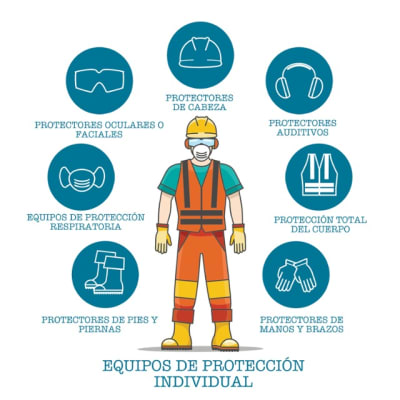
\includegraphics[width=.49\linewidth]{images/epp.jpg}
  \caption{Equipos de protección personal individual.}
  \label{fig:epp}
\end{figure}

\subsection{Uso del Casco de Seguridad}

El casco es uno de los elementos más importantes del EPP \cite{martinez2017aplicacion}, diseñado como se muestra en la figura \ref{fig:casco} para proteger la cabeza del trabajador de impactos con objetos que caen o golpean. Según las normativas internacionales y locales, su uso es obligatorio en prácticamente todas las actividades dentro de una obra. Sin embargo, su efectividad depende del uso correcto y constante. La supervisión del cumplimiento de esta medida es uno de los principales retos en las obras, y es donde las tecnologías emergentes pueden marcar la diferencia.

\begin{figure}[!ht]
  \centering
  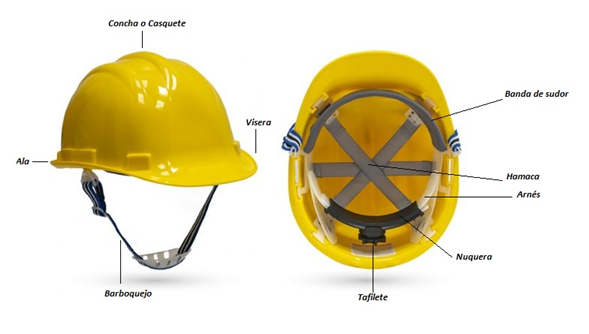
\includegraphics[width=.49\linewidth]{images/casco.png}
  \caption{Estructura de un casco de seguridad.}
  \label{fig:casco}
\end{figure}

\section{Inteligencia Artificial y Visión por Computadora}

\subsection{Definición y Conceptos Básicos}

Según los autores en su libro \cite{russell2016artificial}  han afirmado que la inteligencia artificial (IA) es interesante, pero no se ha definido qué es exactamente. A lo largo de la historia, los investigadores han seguido distintas versiones de la IA. Algunos la han definido en términos de su fidelidad al rendimiento humano, mientras que otros han optado por una definición más abstracta y formal conocida como racionalidad, que, de manera general, se refiere a ``hacer lo correcto''. Además, el enfoque en torno a la inteligencia varía: algunos la consideran una propiedad de los procesos internos de pensamiento y razonamiento, mientras que otros se centran en el comportamiento inteligente, una característica externa.

De estas dos dimensiones —humano vs. racional y pensamiento vs. comportamiento— surgen cuatro combinaciones posibles, y han existido defensores y programas de investigación para cada una. Los métodos utilizados también difieren: el estudio de la inteligencia similar a la humana debe, en parte, ser una ciencia empírica relacionada con la psicología, que implica observaciones e hipótesis sobre el comportamiento y los procesos mentales humanos. Por otro lado, el enfoque racionalista emplea una combinación de matemáticas e ingeniería, y se vincula con la estadística, la teoría del control y la economía. Los diferentes grupos han criticado y también colaborado entre sí. Ahora se examinarán con mayor detalle estas cuatro aproximaciones.

La inteligencia artificial (IA) es una rama de la informática que busca crear sistemas capaces de realizar tareas que normalmente requieren inteligencia humana, como el reconocimiento de patrones, la toma de decisiones y la predicción. La visión por computadora es un subcampo de la IA que se enfoca en permitir que las máquinas “vean” e interpreten el entorno a través de imágenes o videos, extrayendo información útil como la identificación de objetos, clasificación de imágenes o análisis de patrones.

\subsection{Detección de Objetos}

Los autores en \cite{zou2023object} la detección de objetos, considerada uno de los problemas más fundamentales y complejos en el ámbito de la visión por computadora, ha ganado un gran interés en los últimos años. A lo largo de las últimas dos décadas, se ha evidenciado un rápido progreso tecnológico en este campo, lo que ha tenido un impacto significativo en toda la disciplina de la visión por computadora. Si las técnicas actuales de detección de objetos son vistas como una revolución impulsada por el aprendizaje profundo, en la década de 1990 se destacaba el pensamiento innovador y el diseño visionario de los primeros enfoques en visión por computadora. Esta investigación revisa exhaustivamente el desarrollo acelerado de la detección de objetos desde una perspectiva histórica, abarcando más de 25 años de evolución (desde los años 90 hasta 2022). En este contexto, se discuten temas clave como los detectores históricos más importantes, los conjuntos de datos utilizados para la detección, las métricas de evaluación, los componentes fundamentales de los sistemas de detección, las técnicas para mejorar la eficiencia y los métodos más avanzados en la actualidad.

La detección de objetos es una técnica dentro de la visión por computadora que se utiliza para localizar e identificar varios objetos dentro de una imagen o un video como se muestra en la figura \ref{fig:object_detection}. Esta técnica combina la clasificación de imágenes con la localización de objetos, indicando en qué área de la imagen se encuentra el objeto. Se han desarrollado múltiples modelos para esta tarea, siendo YOLO (You Only Look Once) uno de los más eficaces y populares debido a su velocidad y precisión.

\begin{figure}[!ht]
  \centering
  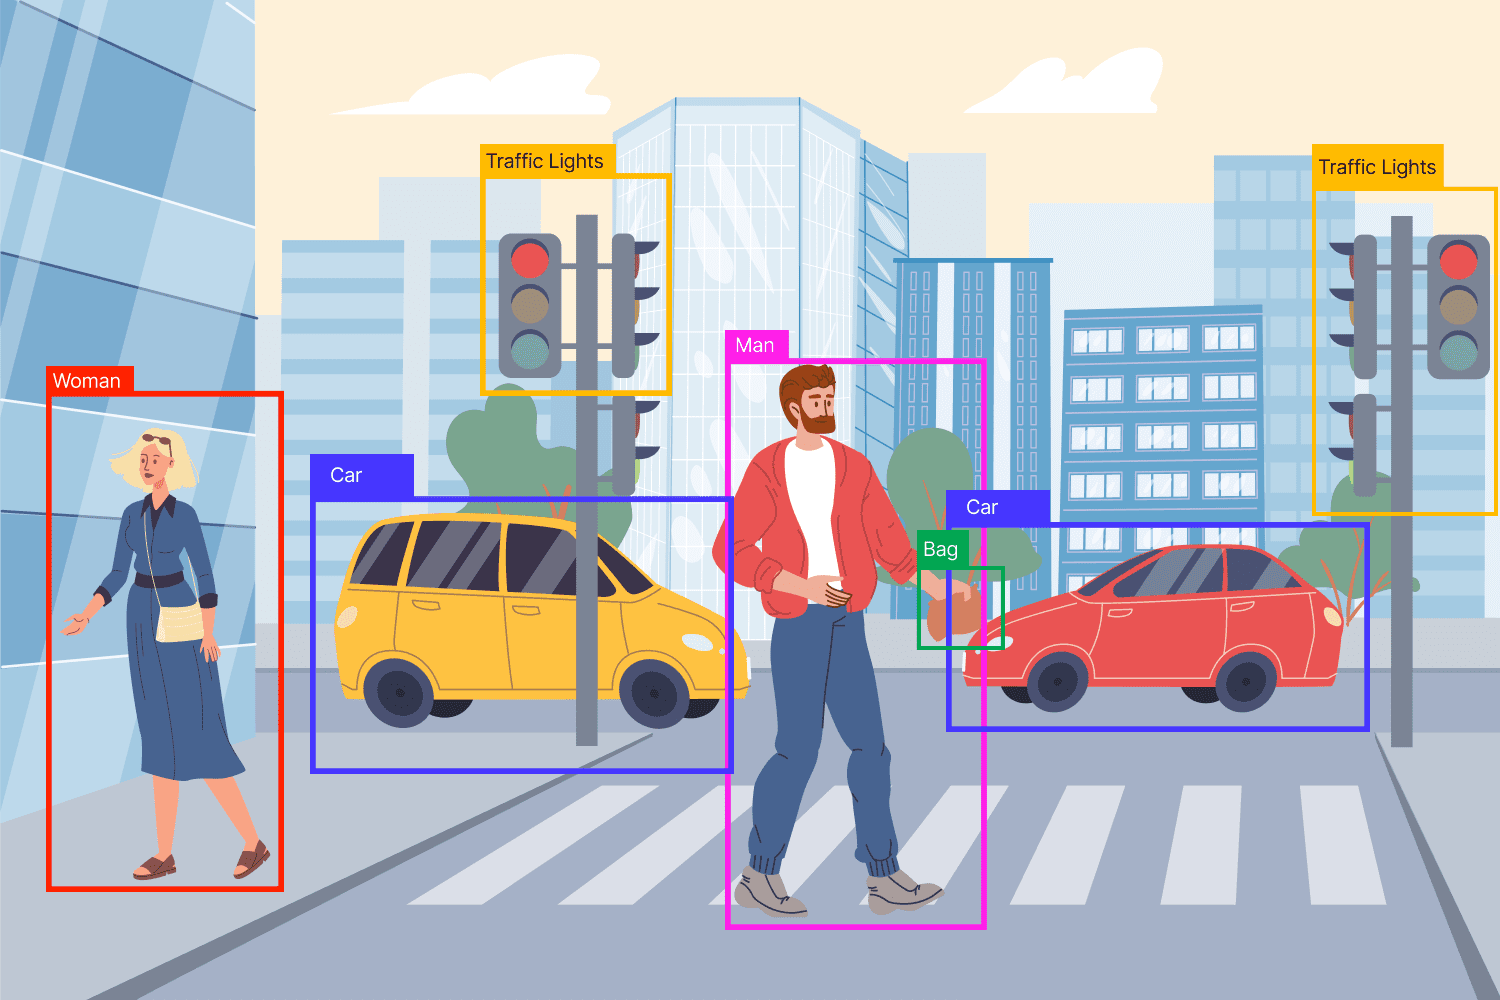
\includegraphics[width=.49\linewidth]{images/object_detection.png}
  \caption{Ejemplo de detección de objetos dentro de una imagen.}
  \label{fig:object_detection}
\end{figure}

\section{Modelos de Detección de Objectos: YOLO}

\subsection{Historia y Evolución de YOLO}

YOLO es una familia de modelos de inteligencia artificial para la detección de objetos en imágenes, creado por Joseph Redmon en 2016. Su principal ventaja radica en su capacidad de detectar objetos en tiempo real con alta precisión, a diferencia de otros modelos que requieren múltiples pasos para lograr este objetivo. Desde su lanzamiento, ha pasado por varias versiones como se muestra en la figura \ref{fig:yolo_evolution}, mejorando en precisión, velocidad y capacidad de generalización en cada iteración. La versión más reciente, YOLOv8, incorpora las últimas innovaciones en redes neuronales profundas.

\begin{figure}[!ht]
  \centering
  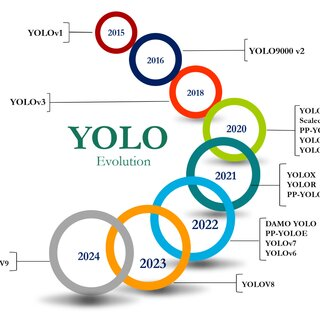
\includegraphics[width=.49\linewidth]{images/yolo_evolution.jpg}
  \caption{Evolución de las versiones de YOLO.}
  \label{fig:yolo_evolution}
\end{figure}

\subsection{Características de YOLOv8}

YOLOv8 es la última versión estable de la serie YOLO \cite{jiang2022review}, y se distingue por su arquitectura optimizada \ref{fig:yolo_architecture}, lo que permite detectar objetos con mayor rapidez y exactitud. Sus principales características incluyen la capacidad de operar en tiempo real, ser más ligero en comparación con sus predecesores, y lograr un balance óptimo entre precisión y velocidad. YOLOv8 ha sido diseñado para integrarse fácilmente en aplicaciones de seguridad, donde la detección precisa y rápida es crucial.

\begin{figure}[!ht]
  \centering
  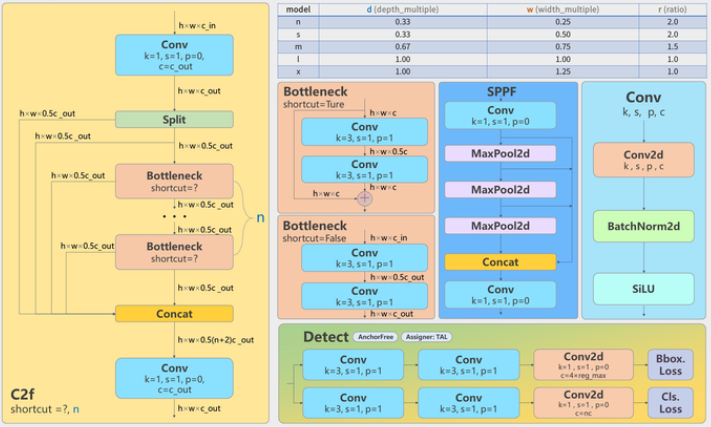
\includegraphics[width=.49\linewidth]{images/yolo_architecture.png}
  \caption{Arquitectura de modelo YOLOv8.}
  \label{fig:yolo_architecture}
\end{figure}

\subsection{Aplicaciones de YOLO en la Seguridad}

El uso de YOLO en el ámbito de la seguridad ha demostrado ser altamente efectivo, especialmente en la detección de equipos de protección personal (EPP) como se muestra en la figura \ref{fig:yolo_application}. En entornos como las obras de construcción, la capacidad de este modelo para detectar la presencia o ausencia de cascos de seguridad en tiempo real representa una herramienta valiosa para mejorar la supervisión y cumplimiento de las normativas de seguridad.

\begin{figure}[!ht]
  \centering
  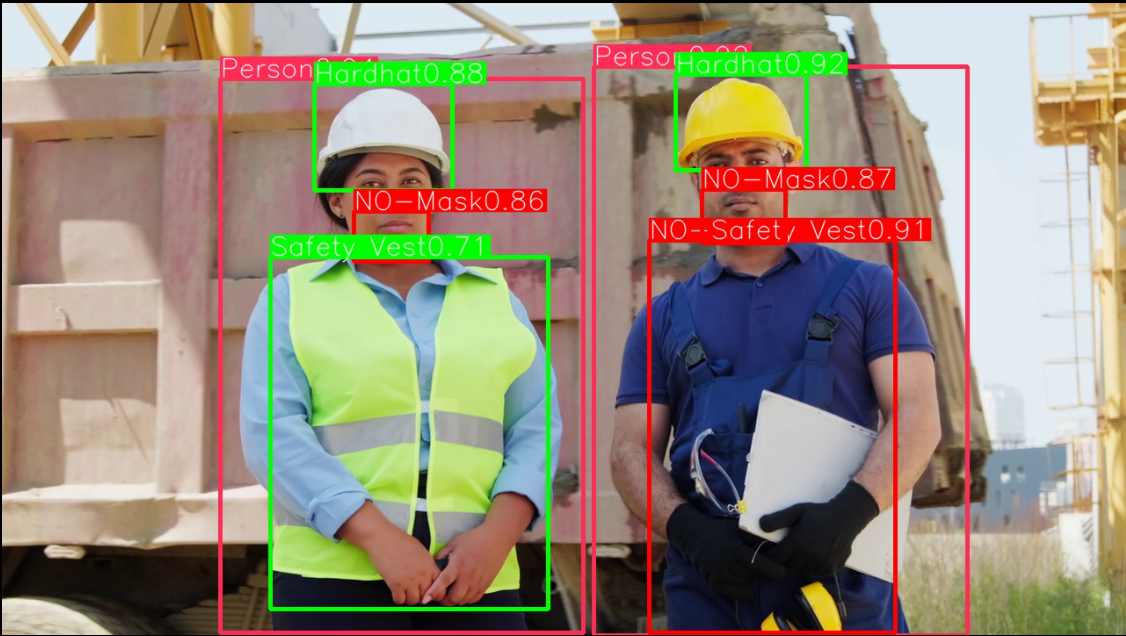
\includegraphics[width=.49\linewidth]{images/yolo_application.png}
  \caption{Aplicación de YOLOv8 en la detección de equipos de protección personal (EPP).}
  \label{fig:yolo_application}
\end{figure}

\section{Técnicas de Preprocesamiento de Imágenes}

\subsection{Redimensionamiento y Recorte de Imágenes}

El redimensionamiento y recorte de imágenes mostrado en la figura \ref{fig:image_cropping} son etapas fundamentales en el preprocesamiento de datos para la detección de objetos. En el caso de YOLOv8, es necesario ajustar las imágenes a un tamaño estándar (640x640 píxeles) para que el modelo pueda procesarlas eficientemente. Se pueden utilizar varias técnicas de recorte, como recorte desde la izquierda, corte centrado, y corte con superposición, para garantizar que todas las áreas importantes de la imagen sean utilizadas.

\begin{figure}[!ht]
  \centering
  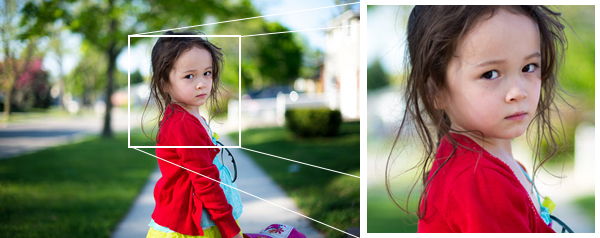
\includegraphics[width=.49\linewidth]{images/cropping.jpg}
  \caption{Recorte de imagen en una región específica.}
  \label{fig:image_cropping}
\end{figure}

\subsection{Aumentación de Datos}

La aumentación de datos es una técnica que se utiliza para expandir el conjunto de datos mediante la creación de variaciones \ref{fig:data_augmentation} de las imágenes originales. Estas variaciones pueden incluir rotaciones, volteos, y cambios en la iluminación. Este proceso ayuda a aumentar la diversidad del dataset, lo que mejora la capacidad del modelo para generalizar y manejar distintos tipos de imágenes.

\begin{figure}[!ht]
  \centering
  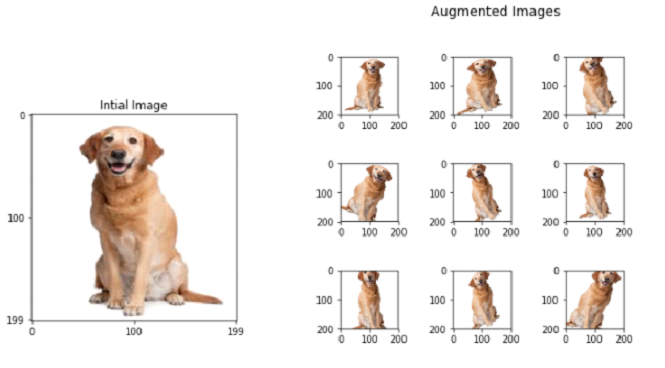
\includegraphics[width=.49\linewidth]{images/data_augmentation.png}
  \caption{Aumentación de imágenes con diferentes configuraciones.}
  \label{fig:data_augmentation}
\end{figure}

\section{Herramientas y Plataformas de Etiquetado}

\subsection{Introducción al Etiquetado de Imágenes}

El etiquetado de imágenes es el proceso mediante el cual se asignan etiquetas o clases a objetos dentro de una imagen. En el caso de los EPPs, se etiqueta la presencia de cascos, lo que permite que el modelo aprenda a reconocer estos elementos. El etiquetado es un paso crucial, ya que los datos mal etiquetados pueden afectar negativamente el rendimiento del modelo.

\subsection{Roboflow: Plataforma de Etiquetado}

Roboflow es una plataforma  \ref{fig:roboflow_labeling} popular para la gestión y etiquetado de imágenes en proyectos de visión por computadora. Ofrece una interfaz intuitiva para cargar, etiquetar y preparar datasets para ser utilizados en modelos como YOLOv8. La plataforma también facilita la exportación de los datos en formatos compatibles con YOLO, optimizando el flujo de trabajo para la creación de modelos personalizados.

\begin{figure}[!ht]
  \centering
  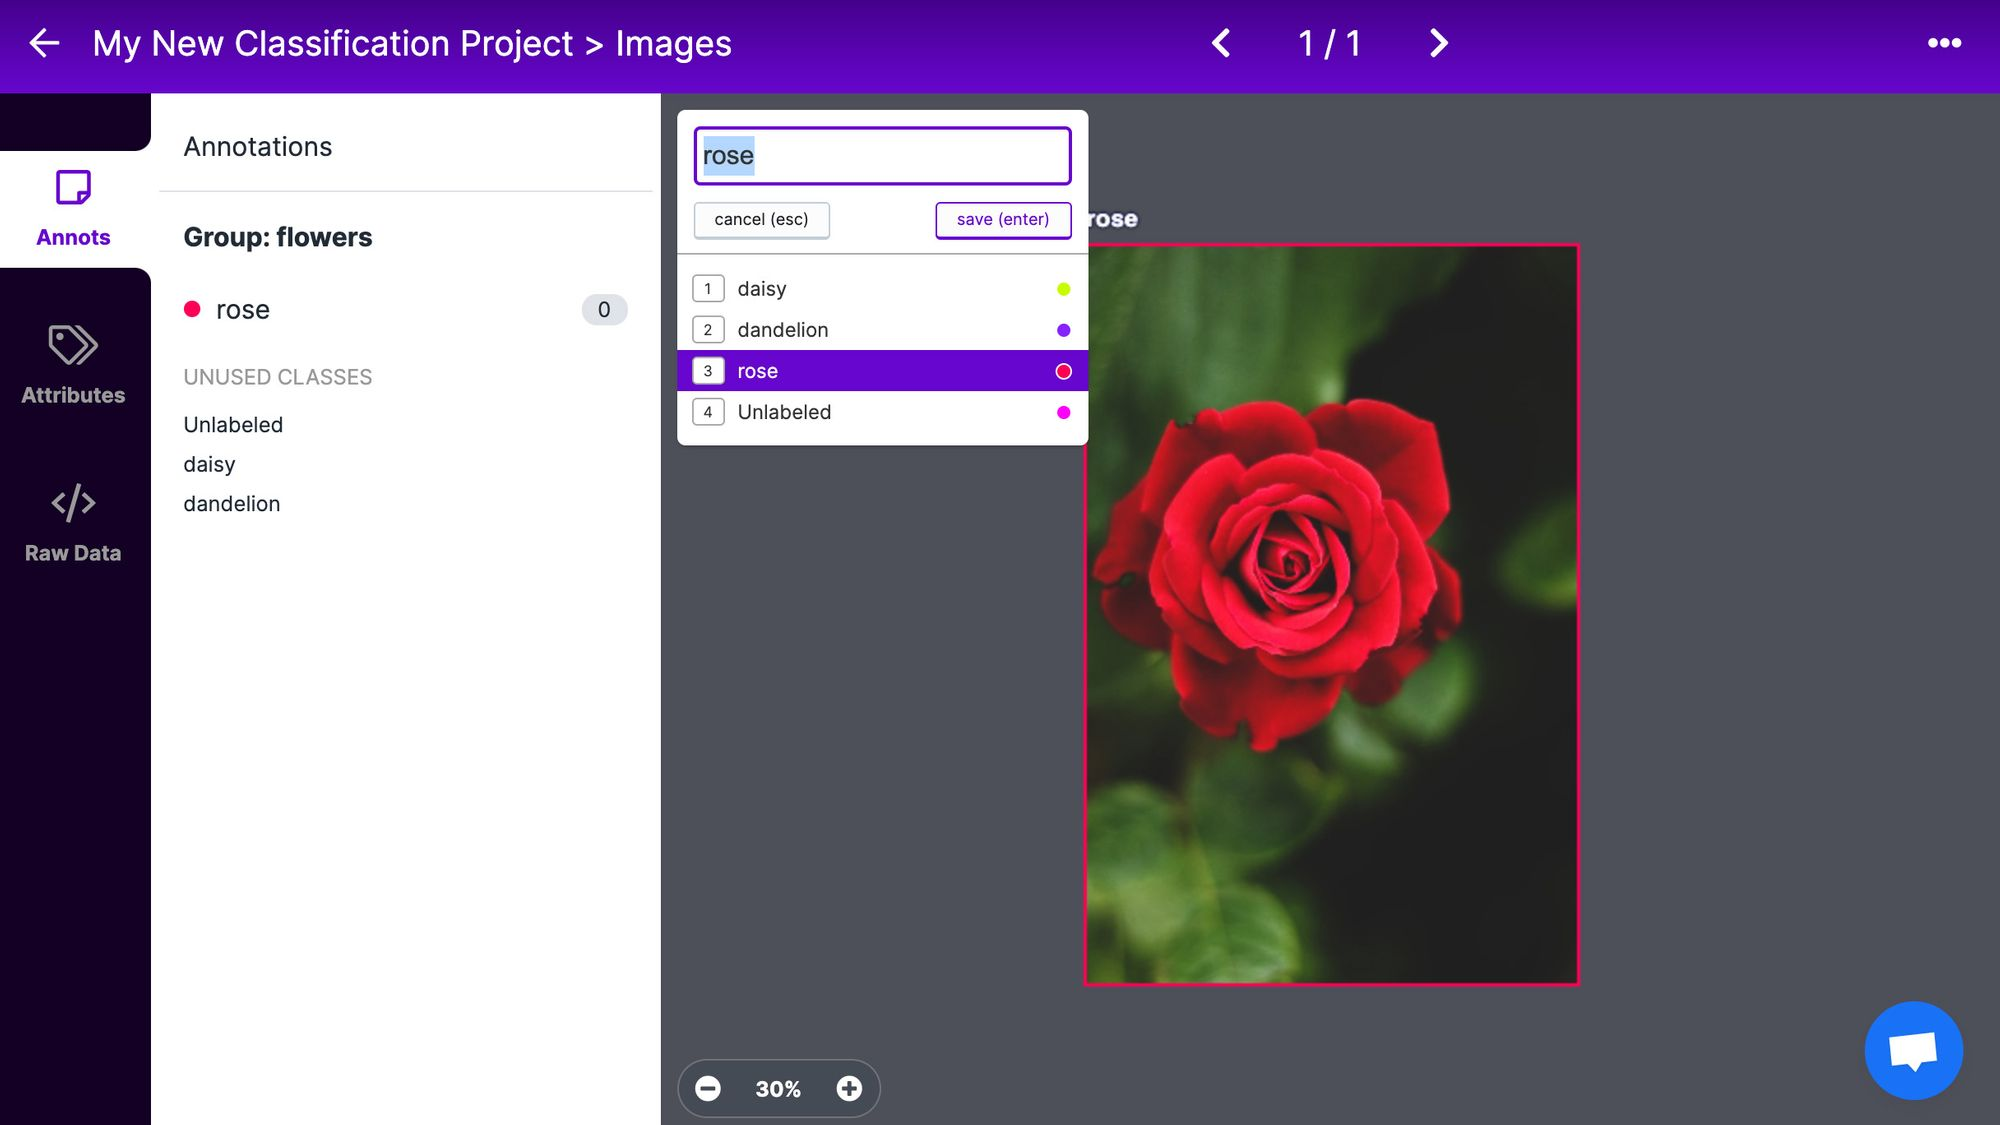
\includegraphics[width=.49\linewidth]{images/roboflow_labeling.jpg}
  \caption{Interfaz de Roboflow para el etiquetado de clases.}
  \label{fig:roboflow_labeling}
\end{figure}




\chapter{METODOLOGÍA DE LA INVESTIGACIÓN}

\section{Enfoque de la Investigación}

La presente investigación tiene un enfoque cuantitativo y experimental, ya que se busca generar un dataset que sirva como entrada para el entrenamiento de un modelo de detección de objetos (YOLOv8) y evaluar su desempeño en la identificación de equipos de protección personal (EPP), específicamente cascos de seguridad, en un entorno de obra real. El enfoque cuantitativo se justifica por la medición de variables como la precisión del modelo y la calidad de las imágenes procesadas, mientras que el enfoque experimental se debe a la implementación y prueba de diferentes algoritmos de corte y técnicas de preprocesamiento de imágenes.

\section{Diseño de la Investigación}

El diseño de la investigación es no experimental, ya que no se manipularán directamente las variables independientes (el uso de cascos de seguridad por parte de los trabajadores). En su lugar, se recolectarán datos a través de la captura de imágenes reales en una obra de construcción, y se procesarán mediante técnicas de visión por computadora. Este diseño incluye un trabajo de campo para la recolección de datos (imágenes de los trabajadores) y un trabajo de laboratorio para el procesamiento, etiquetado y análisis del dataset.

\section{Recolección de Datos}

\subsection{Selección del Sitio de Estudio}

La obra seleccionada para la toma de imágenes es el proyecto denominado ``COMERCIO''. Se eligió este entorno porque refleja condiciones reales de trabajo en construcción, donde los trabajadores utilizan equipos de protección personal, incluyendo cascos de seguridad. Se solicitó previamente el permiso necesario para acceder a la obra y realizar la toma de fotografías sin interferir con las actividades de la obra.

La obra está ubicada en la región de Arequipa, en el distrito de Cono Norte, Asentamiento Poblacional Asociación de Pequeños Industriales y Artesanos Arequipa APPIAR Mz N Lotes 1.

\begin{figure}[!ht]
  \centering
  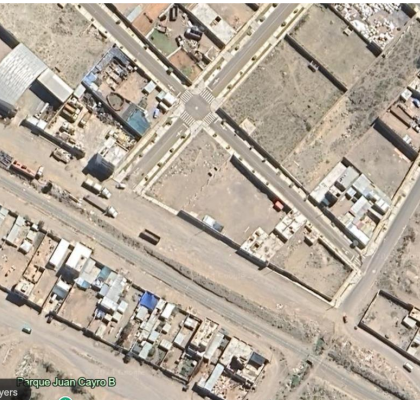
\includegraphics[width=.49\linewidth]{images/comercio.png}
  \caption{Ubicación referencial de la obra ``Comercio''.}
  \label{fig:comercio}
\end{figure}

\subsection{Equipamiento Utilizado}

Para la captura de las imágenes, se utilizó un dispositivo móvil de la maraca Honor X8a \ref{fig:honor} con sistema operativo Android, con una cámara que permite obtener fotografías de alta resolución con dimensiones de 5992x4344 píxeles. Este equipo fue seleccionado por su facilidad de uso y su disponibilidad para capturar imágenes de manera espontánea en el entorno de la obra.

\begin{figure}[!ht]
  \centering
  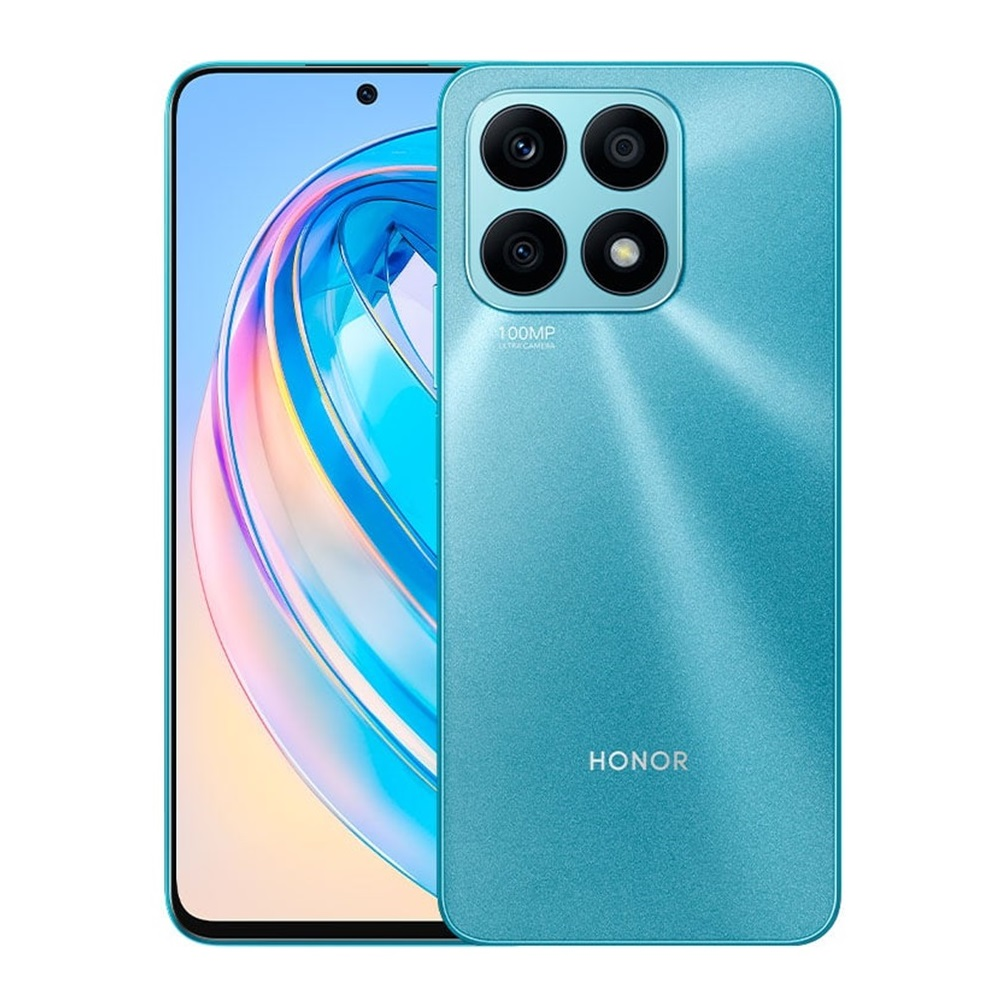
\includegraphics[width=.49\linewidth]{images/honor.jpg}
  \caption{Dispositivo movil Honor X8a utilizado para la toma de fotografías.}
  \label{fig:honor}
\end{figure}

\subsection{Proceso de Captura de Imágenes}

Se realizaron capturas de imágenes durante varias jornadas de trabajo en la obra, con el objetivo de obtener imágenes variadas de los trabajadores en diferentes situaciones, ángulos y posiciones. Las imágenes fueron tomadas en condiciones naturales de la obra, sin preparación previa de los trabajadores, con el fin de reflejar un entorno real. Se tomaron un total de 66 fotografías \ref{fig:photos} en distintas ubicaciones y con diferentes grupos de trabajadores, priorizando situaciones donde el uso de cascos de seguridad fuera evidente.

\begin{figure}[!ht]
  \centering
  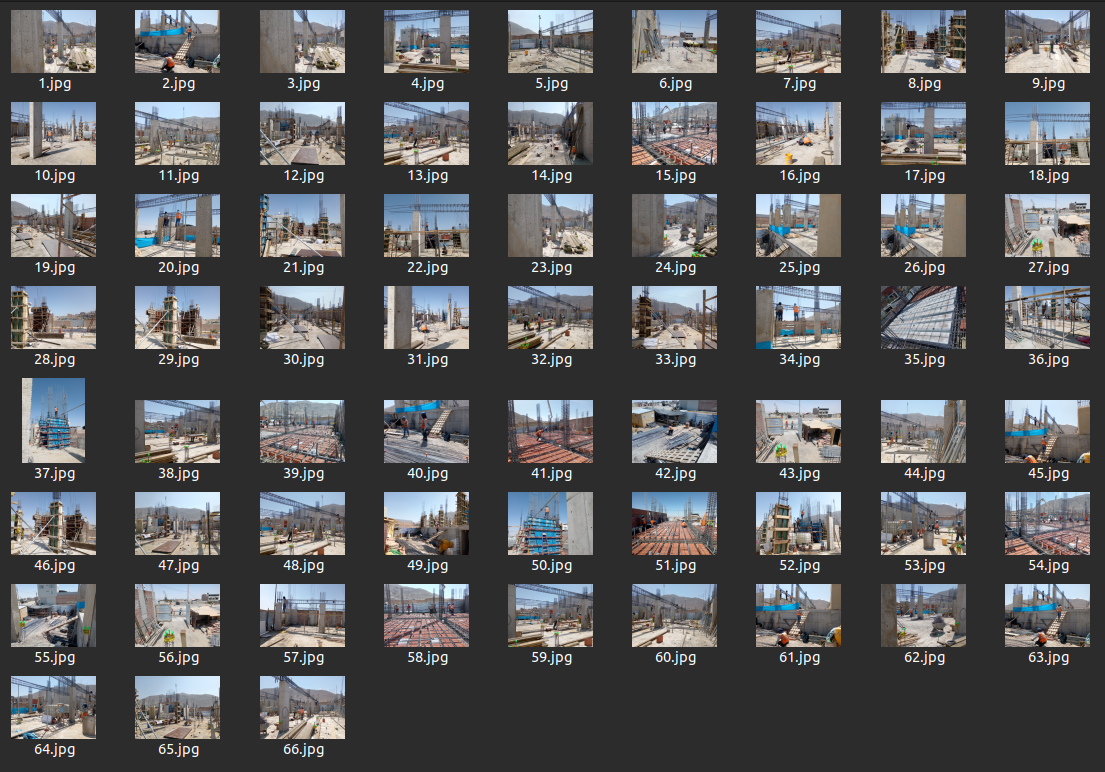
\includegraphics[width=.49\linewidth]{images/photos.png}
  \caption{66 fotografia tomadas en la obra ``Comercio''.}
  \label{fig:photos}
\end{figure}

\section{Preprocesamiento de los Datos}

\subsection{Redimensionamiento de Imágenes}

Las imágenes capturadas originalmente con una resolución de 5992x4344 píxeles fueron redimensionadas a 640x640 píxeles, que es el tamaño estándar requerido por el modelo YOLOv8 para su entrenamiento. Este proceso de redimensionamiento se llevó a cabo utilizando tres algoritmos diferentes de corte:

\begin{itemize}
  \item \textbf{Recorte desde la izquierda:} Se inicia el recorte de las imágenes desde el borde superior izquierdo, generando múltiples imágenes de 640x640 píxeles hasta cubrir el área de la imagen original. Se deja un residuo en la parte final derecha con una dimension menor a 640 pixeles, de la misma manera en la parte inferior como se muestra en la figura \ref{fig:left_cropping}.

\begin{figure}[!ht]
  \centering
  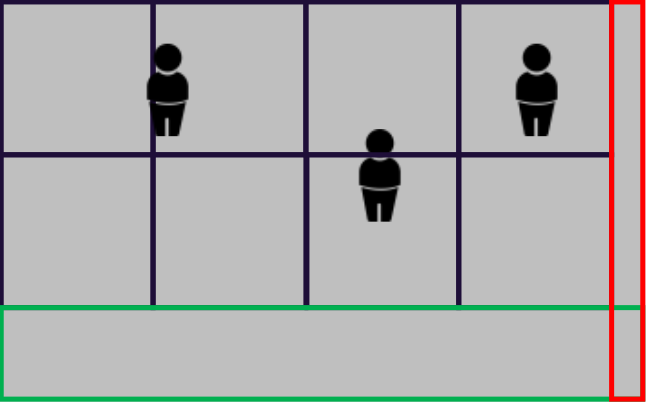
\includegraphics[width=.49\linewidth]{images/left_cropping.png}
  \caption{Esquema de recorte desde la izquierda.}
  \label{fig:left_cropping}
\end{figure}

\item \textbf{Recorte centrado:} El recorte se realiza dividiendo el residuo de la imagen original entre los bordes izquierdo y derecho, así como entre el borde superior e inferior, para centrar la imagen de 640x640 píxeles en la escena como se muestra en la figura \ref{fig:center_cropping}.

\begin{figure}[!ht]
  \centering
  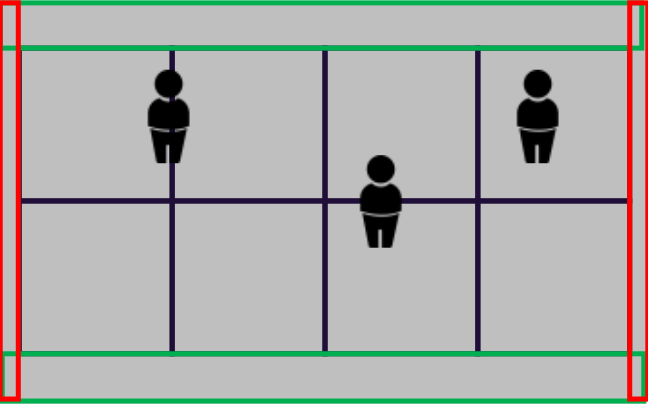
\includegraphics[width=.49\linewidth]{images/center_cropping.png}
  \caption{Esquema de recorte centrado.}
  \label{fig:center_cropping}
\end{figure}

\item \textbf{Recorte con superposición:} Se recortan imágenes de 640x640 píxeles con una pequeña porción de superposición entre ellas, generando imágenes adicionales para asegurar que todos los objetos presentes en la escena original estén representados como se muestra en la figura \ref{fig:full_cropping}.

\begin{figure}[!ht]
  \centering
  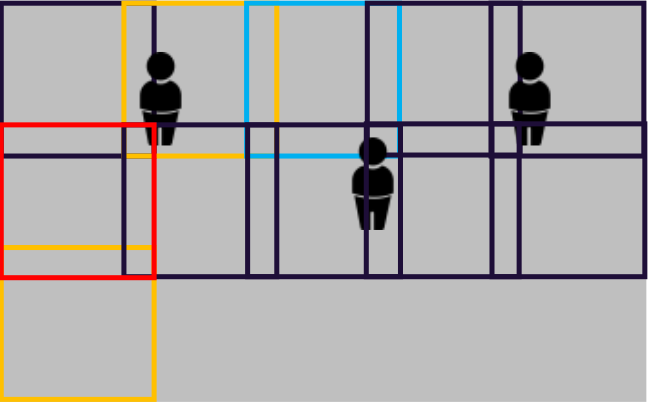
\includegraphics[width=.49\linewidth]{images/full_cropping.png}
  \caption{Esquema de recorte con superposición.}
  \label{fig:full_cropping}
\end{figure}

\end{itemize}

\subsection{Filtrado de Imágenes}

Tras el proceso de recorte, no todas las imágenes contenían personas o trabajadores utilizando EPP. Para filtrar las imágenes sin relevancia, se utilizó un modelo YOLOv8m preentrenado, que detectó la presencia de personas en las imágenes recortadas. A aquellas imágenes que no contenían personas se les aplicó un filtro adicional con el modelo YOLOv8x, con un umbral de confianza del 90\%, para garantizar que las imágenes restantes contenían trabajadores en escenas donde el uso de cascos pudiera ser detectado. De esta manera, el dataset final se redujo a 642 imágenes útiles.

\subsection{Aumentación de Datos}

Para mejorar la generalización del modelo YOLOv8 durante el entrenamiento, se aplicaron técnicas de aumentación de datos utilizando la librería Keras. Se aplicaron las siguientes transformaciones a las imágenes:

\begin{itemize}
  \item \textbf{Rotación aleatoria (RandomRotation):}  Se rotaron las imágenes hasta un máximo del 10\% de 360 grados centrigrados, lo que introduce variabilidad en los ángulos de las imágenes.
  \item \textbf{Volteo horizontal (RandomFlip):} Se aplicó un volteo horizontal aleatorio a las imágenes.
\end{itemize}


\section{Etiquetado de Imágenes}

El etiquetado de las imágenes se llevó a cabo en la plataforma Roboflow como se muestra en la figura \ref{fig:roboflow_use}, una herramienta especializada para el etiquetado. Se creó un proyecto denominado ``helmet detection'', donde se cargaron las 1248 imágenes procesadas y aumentadas. Cada imagen fue revisada manualmente para etiquetar los cascos de seguridad, asignándoles la clase \textit{``helmet''} en el formato compatible con YOLOv8.

\begin{figure}[!ht]
  \centering
  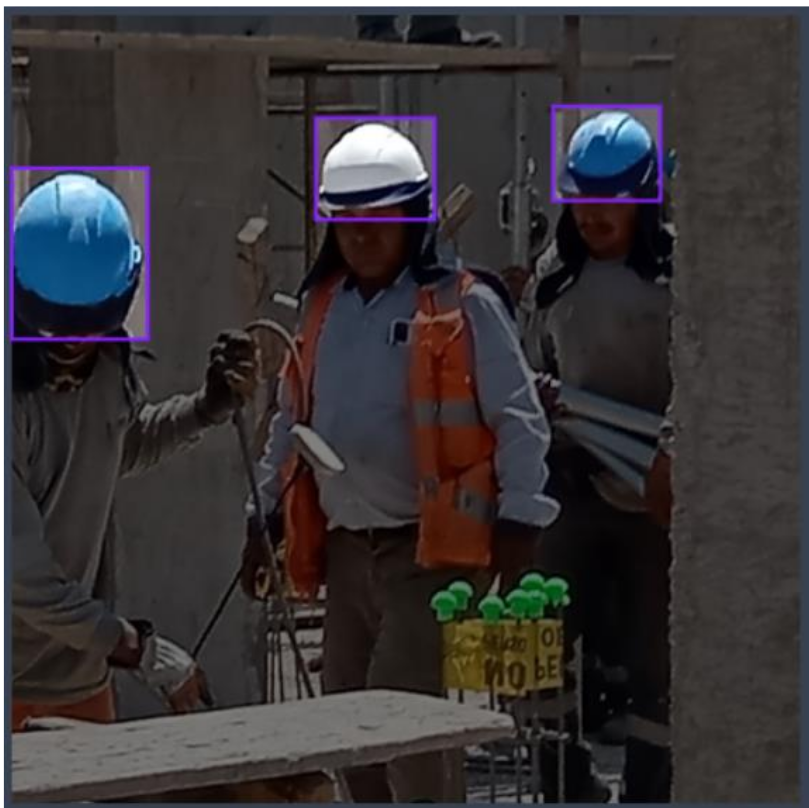
\includegraphics[width=.49\linewidth]{images/roboflow_use.png}
  \caption{Uso de la plataforma Roboflow para el etiquetado de la clase \textit{helmet}.}
  \label{fig:roboflow_use}
\end{figure}


\chapter{RESULTADOS Y DISCUSION}

\section{Resultados de Imagenes Recortadas}

\subsection{Resultados de Recorte por la Izquierda}

El procedimiento se realiza el recorte se explicó en el item 3.4.1. Los resultados obtenidos mediante esta tecnica se muestra en la figura \ref{fig:left_use}.

\begin{figure}[!ht]
  \centering
  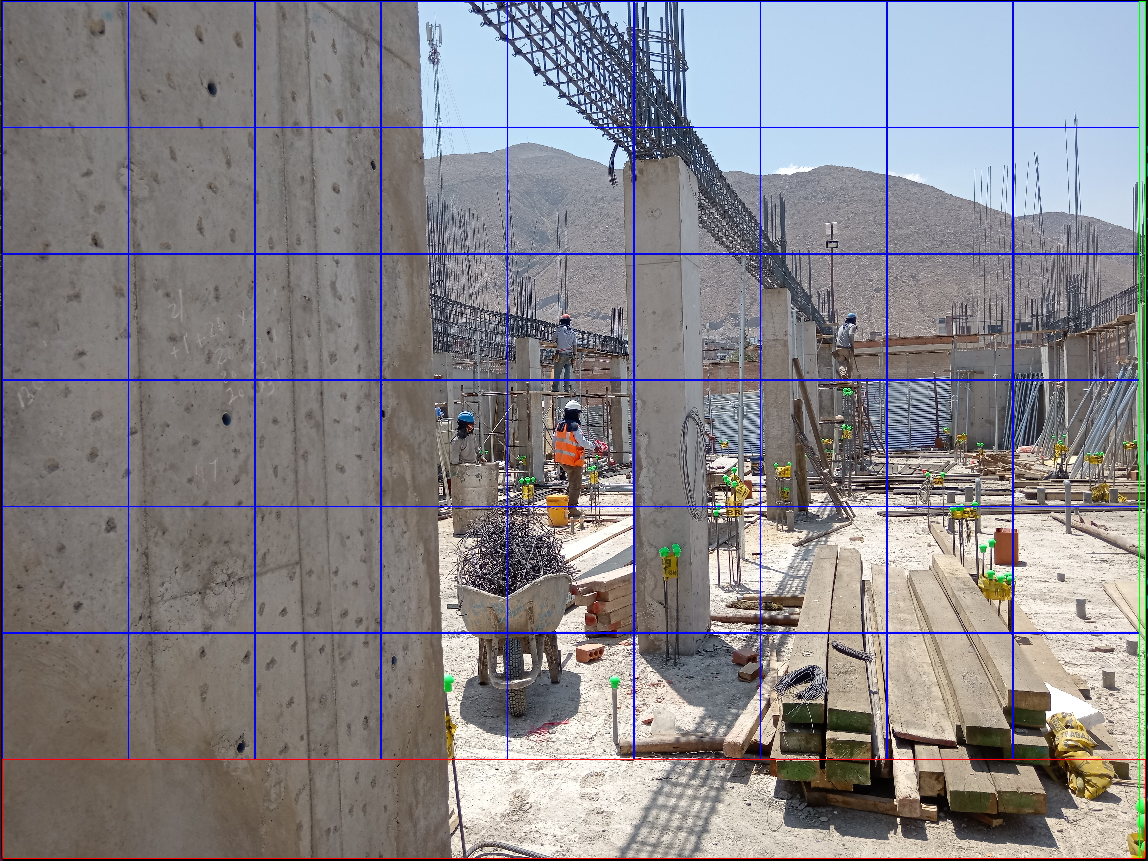
\includegraphics[width=.49\linewidth]{images/left_use.png}
  \caption{Ejemplo de resultado obtenido mediante el recorte por la izquierda.}
  \label{fig:left_use}
\end{figure}

\subsection{Resultados de Recorte Centrado}

Los resultados obtenidos mediante la tecnica de recorte centrado se muestra en la siguiente figura \ref{fig:center_use}.

\begin{figure}[!ht]
  \centering
  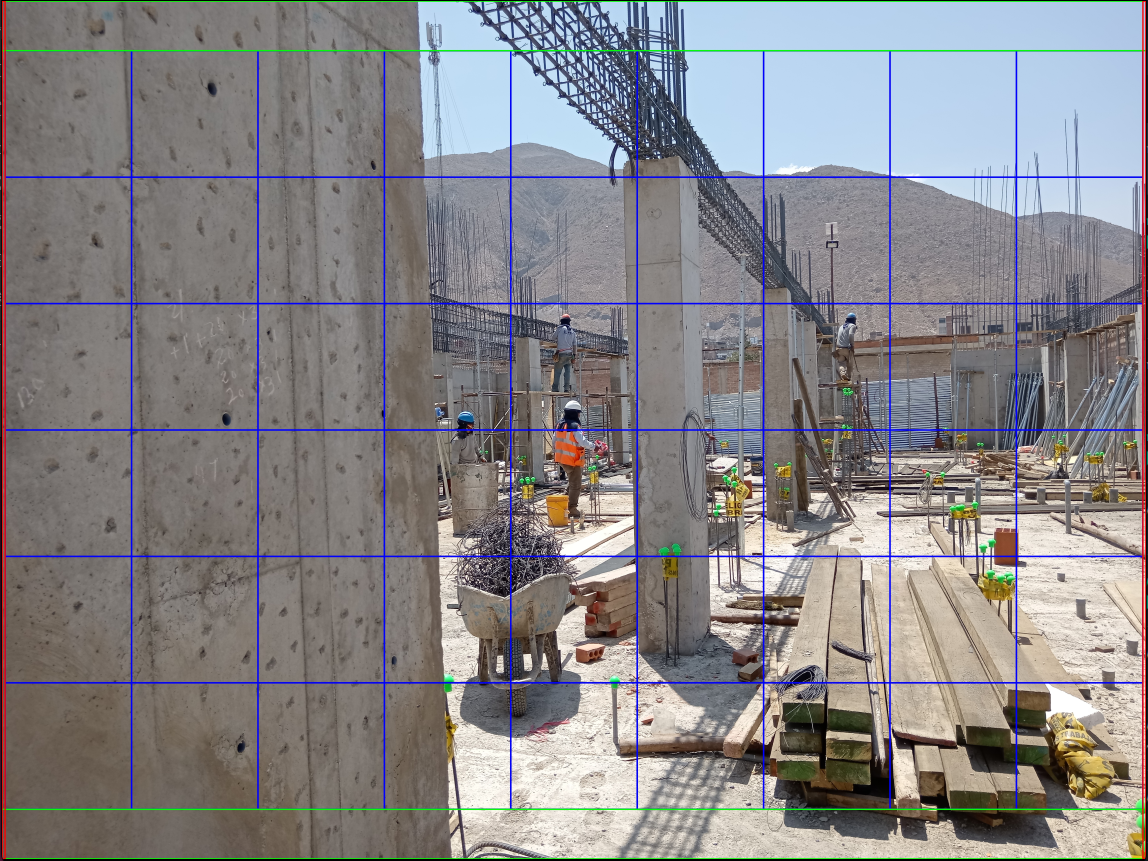
\includegraphics[width=.49\linewidth]{images/center_use.png}
  \caption{Ejemplo de resultado obtenido mediante el recorte centrao.}
  \label{fig:center_use}
\end{figure}

\subsection{Resultados de Recorte Superpuesto}

Los resultados obtenidos medainte la tecnica de recorte superpuesto se muestra en la siguiente figura \ref{fig:full_use}.

\begin{figure}[!ht]
  \centering
  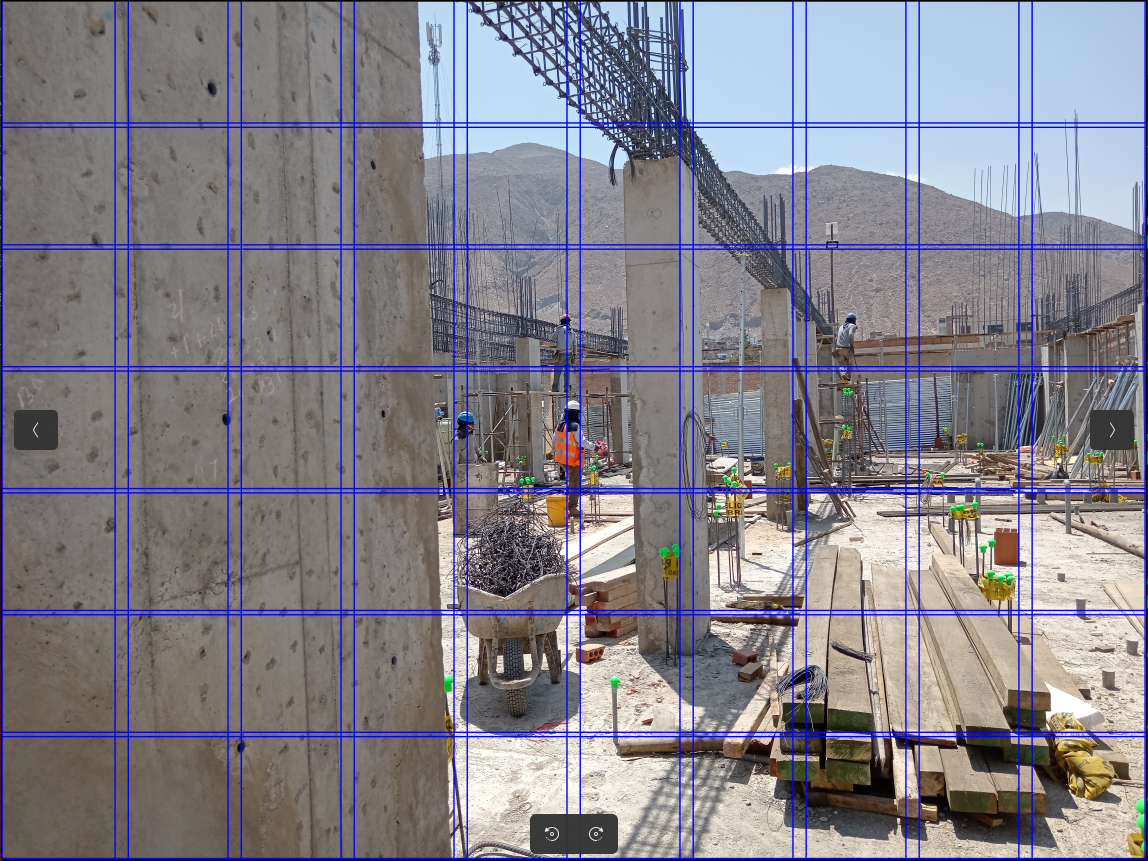
\includegraphics[width=.49\linewidth]{images/full_use.png}
  \caption{Ejemplo de resultado obtenido mediante el recorte superpuesto.}
  \label{fig:full_use}
\end{figure}

\subsection{Resultados de Recorte por Reconocimiento}

Los resultados obtenidos mediante la tecnica de reconocimiento con el modelo preentrenado de yolov8m. El recorte se realizo a partir de la deteccion del centro de la persona detectada, dandole las dimensiones de 640x640 pixles.

\subsection{Resumen Segun las Tecnicas de Recorte}

La siguiente tabla \ref{tab:summary_table} muestra el resultado de haber utilizado 4 tecnicas de recorte de imagenes.

\begin{table}[ht]
  \centering
  \begin{tabular}{|l|c|c|}
      \hline
       & \textbf{Antes del filtro}  & \textbf{Despues del filtro}\\ \hline
      \textbf{Recorte por izquierda} & 3564 & 469 \\ \hline
      \textbf{Recorte centrado} & 3564 & 493 \\ \hline
      \textbf{Recorte superpuesto} & 4221 & 503 \\ \hline
      \textbf{Recorte con yolov8} & - & 289 \\ \hline
      \textbf{total} & \textbf{11349} & \textbf{1754} \\ \hline
  \end{tabular}
  \caption{Cantidad de imagenes despues de aplicar las 4 tecnicas de recorte antes del filtrado y despues del filtrado.}
  \label{tab:summary_table}
\end{table}

\subsection{Resultado Final Obtenido}

El resultado final obtenido despues de aplicar el primer filtro con la configuracion por defecto del modelo  preentrenado yolov8m, el segundo filtro con un nivel de confianza del 90\% del modelo preentrenado yolov8x y finalmente la tecnica de aumentacion de datos se muestra en el siguiente cuadro \ref{tab:final_report}.

\begin{table}[ht]
  \centering
  \begin{tabular}{|l|c|c|}
      \hline
       & \textbf{Total de imagenes} \\ \hline
      \textbf{Primer filtro} & 1754 \\ \hline
      \textbf{Segundo filtro} & 624 \\ \hline
      \textbf{Aumentación de datos} & 1248 \\ \hline
  \end{tabular}
  \caption{Cantidad de imagenes obtenidos despues de las tecnicas de filtro y aumentacion de datos.}
  \label{tab:final_report}
\end{table}


\chapter*{CONCLUSIONES}
\addcontentsline{toc}{chapter}{CONCLUSIONES}

\begin{itemize}
  \item Se concluye que los modelos de detección de objetos entrenados con datos generados en entornos controlados son poco eficientes al momento de hacer uso en el campo real.
  \item Las técnicas de recorte por izquierda, centrado y superpuesto son eficientes para detectar instancias alejadas en la imagen original, sin embargo, la técnica por reconocimiento es eficiente para instancias cercanas en la imagen.
  \item Después de realizado el primer filtrddo con el modelo yolov8m preentrenado con una configuración por defecto se redujo en un total 84.5\% obteniendose 1754 imágenes de un total de 11349 imágenes recortadas.
  \item Por otro lado afirmamos que la técnica de recorte superpuesto es mas eficiente, esto debido a que se obtuvo mayor cantidad de imagenes con instancias de personas, con el cual se obtuvo 503 imágenes.
  \item Al realizar un segundo filtrado con un umbral de confianza del 90\% se redujo en un 64.4\% con respecto al primer filtrado y un 94.5\% con respecto al total de imágenes obtenidas después de los recoretes.
  \item Por último al hacer uso de un modelo preentrenado de yolov8 para realizar los filtros mediante la detección de personas en las imágenes recortadas, este confunde algunos objetos con personas, dando como resultado imágenes sin personas.
\end{itemize}
\chapter*{RECOMENDACIONES}
\addcontentsline{toc}{chapter}{RECOMENDACIONES}

\begin{itemize}
  \item Para el uso de modelos de detección de objetos en aplicaciones reales se recomienda realizar tecnicas de \textit{``transfer learning''} de modelos ya entrenados con datos que reflejan el campo real.
  \item Así mismo, se recomienda generar un dataset con datos lo más cercano al objetivo de aplicación.
  \item Se recomienda hacer uso de \textit{softwares} de edición de imágenes para realizar el recorte de imágenes.
  \item También se recomienda verificar la efectividad de la técnida \textit{``data augmentation''} probando diferentes configuraciones y entrenando un modelo con los mismos datos.
\end{itemize}

% Bibliography
\printbibliography
\addcontentsline{toc}{chapter}{BIBLIOGRAFÍA}


\end{document}